\subsection{Struktura wirtualnego efektora}
\label{subsec:ve-gripper-struktura}

\begin{figure}[ht]
    \centering
    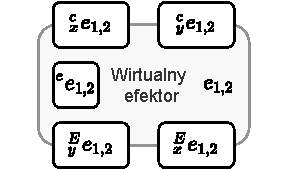
\includegraphics[width=0.75\columnwidth]{figures/ISR-ve-gripper-model.pdf}
    \caption{Struktura ogólna wirtualnego efektora chwytaka dwustanowego}
    \label{fig:model-ve-gripper}
\end{figure}

Na rysunku~\ref{fig:model-ve-gripper} przedstawiono widok wirtualnego efektora chwytaka dwustanowego w~projektowanym systemie. Jego rolą jest nadzorowanie pracą rzeczywistego efektora sterującego chwytakiem. Do poprawnej pracy podsystemu wymagane są wszystkie cztery bufory komunikacyjne, jednak nie potrzebuje on do działania wewnętrznej pamięci. Podobnie jak efektor manipulatora, krok dyskretyzacji został ustawiony na ${}^{e}T = \frac{1}{30}s$.

\subsubsection{Bufory komunikacyjne}
\begin{itemize}
    \item ${}^{c}_{x}e_{1,2} = \xi_{\mathrm{zad}} \in \{o, c\}$ - zadany stan chwytaka,
    \item ${}^{c}_{y}e_{1,2} = \xi \in \{o, c\}$ - aktualny stan chwytaka przesyłany do podsystemu sterowania,
    \item ${}^{E}_{x}e_{1,2} = \Xi \in \{o, c\}$ - aktualny stan chwytaka, aktualizowany po pełnym rozwarciu chwytaka lub po maksymalnym domknięciu,
    \item ${}^{E}_{y}e_{1,2} = \Xi_{\mathrm{zad}} \in \{o, c\}$ - aktualnie realizowany stan chwytaka.
\end{itemize}

\subsection{Automat sterujący}
Prostota działania chwytaka implikuje jeden stan normalnej pracy urządzenia, z~którym skojarzone zostało zachowanie ${}^{e}\mathcal{B}_{1,2,0}$ (\textbf{work}). Zachowanie \textbf{work} jest jedynym zachowaniem podsystemu, dlatego nie ma potrzeby rozważania warunków początkowych oraz końcowych. 

Automat sterujący chwytakiem składa się z~tylko jednego stanu, co implikuje że warunek początkowy jest zawsze spełniony, natomiast warunek końcowy nigdy nie jest spełniony. Oznacza to że dla takiego automatu są spełnione warunki kompletności oraz rozłączności warunków stanów następnych.

\subsubsection{Funkcja przejścia}
\begin{equation}
    \begin{gathered}
        {}^{e_{1,2}, E_{1,2}}f_{1,2,0} \triangleq {}^{E}_{y}e_{1,2} = \xi,\\
        {}^{e_{1,2}, c_{1,1}}f_{1,2,0} \triangleq {}^{c}_{y}e_{1,2} = \Xi
    \end{gathered}
\end{equation}

\begin{figure}
    \centering
    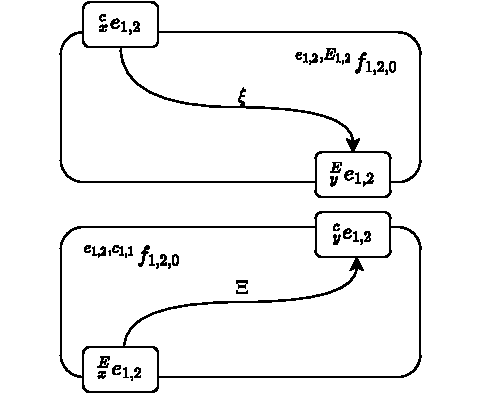
\includegraphics[width=\columnwidth]{figures/ISR-ve-gripper-fp-work.pdf}
    \label{fig:ve-gripper-fp-work}
    \caption{Zdekomponowana funkcja przejścia zachowania \textbf{work} w~postaci DFD}
\end{figure}


%%%%%%%%%%%%%%%%%%%%%%%%%%%%%%%%%%%%%%%%%%%%%%%%%%%%%%%%%%%%%%%%%%%%%%%%%%%%%%%%%